\chapter{Interface Utilisateur et Scénarios d'Exploitation}
\label{chap:interface_ui}

\section{Architecture Ergonomique et Principes Réactifs}

L'interface graphique du moteur CBIR (\texttt{frontend/app.py}) est développée avec le cadriciel réactif \textbf{Streamlit}. L'ergonomie a été spécialement étudiée pour concilier la simplicité de manipulation pour un utilisateur néophyte et le contrôle algorithmique granulaire attendu par un ingénieur ou un chercheur en vision par ordinateur.

La persistance de l'état entre les ré-exécutions réactives du script est assurée par le dictionnaire \texttt{st.session\_state}. La feuille de style CSS injectée personnalise un thème sombre contemporain (\textit{Modern Dark Theme}) structuré autour de contrastes nets, de cartes avec micro-interactions au survol (\textit{hover effect}) et de badges colorés proportionnels à la distance métrique.

\begin{figure}[H]
    \centering
    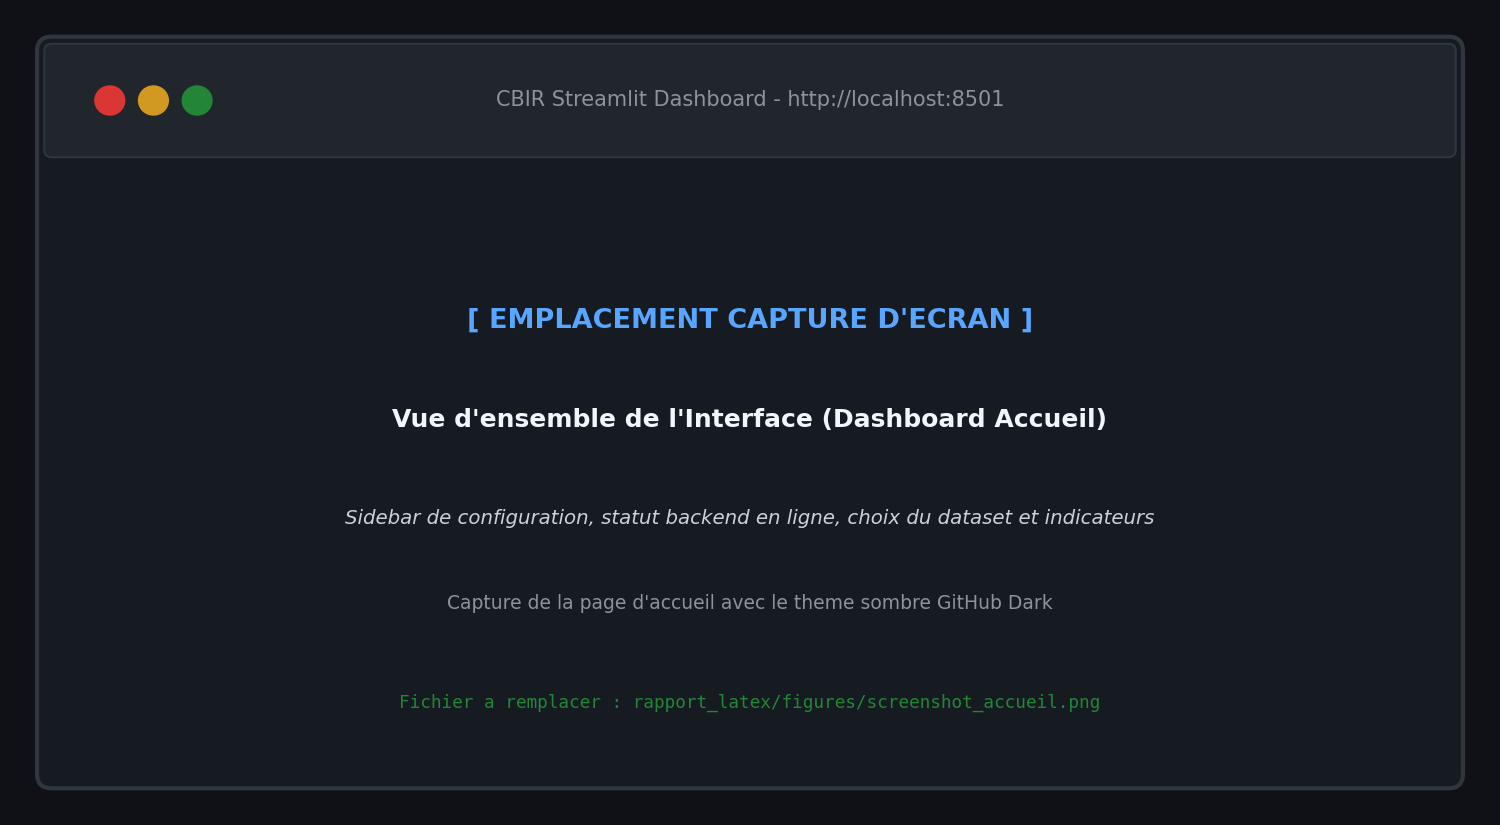
\includegraphics[width=0.92\textwidth]{figures/screenshot_accueil.png}
    \caption{Emplacement Capture 1 : Vue générale du tableau de bord CBIR (Sidebar de configuration, état du backend, sélecteur de collections et indicateurs).}
    \label{fig:screen_accueil}
\end{figure}

\section{Scénario d'Exploitation 1 : Recherche Textuelle et Tolérance Floue}

\subsection{Cas A : Recherche par Mot-Clé Exact}
\textbf{Objectif utilisateur :} Retrouver rapidement l'ensemble des spécimens photographiques appartenant à la catégorie des papillons.

\textbf{Déroulement opérationnel :}
\begin{enumerate}[nosep]
    \item Dans la barre latérale, l'utilisateur sélectionne le mode \textbf{Texte} et le dataset \textbf{objects}.
    \item Dans le champ de recherche central, il saisit le terme \texttt{"butterfly"}.
    \item Il clique sur le bouton \textbf{« 🔍 Rechercher »} (ou valide par la touche Entrée).
\end{enumerate}

\textbf{Comportement système :} L'API évalue la requête via \texttt{POST /api/search/text}. Le moteur SQLite effectue un filtrage SQL conjonctif sur \texttt{category LIKE '\%butterfly\%'}. Les $k = 20$ résultats sont retournés en moins de $15$ millisecondes et affichés sous forme d'une grille réactive à 4 colonnes (figure \ref{fig:screen_texte}).

\begin{figure}[H]
    \centering
    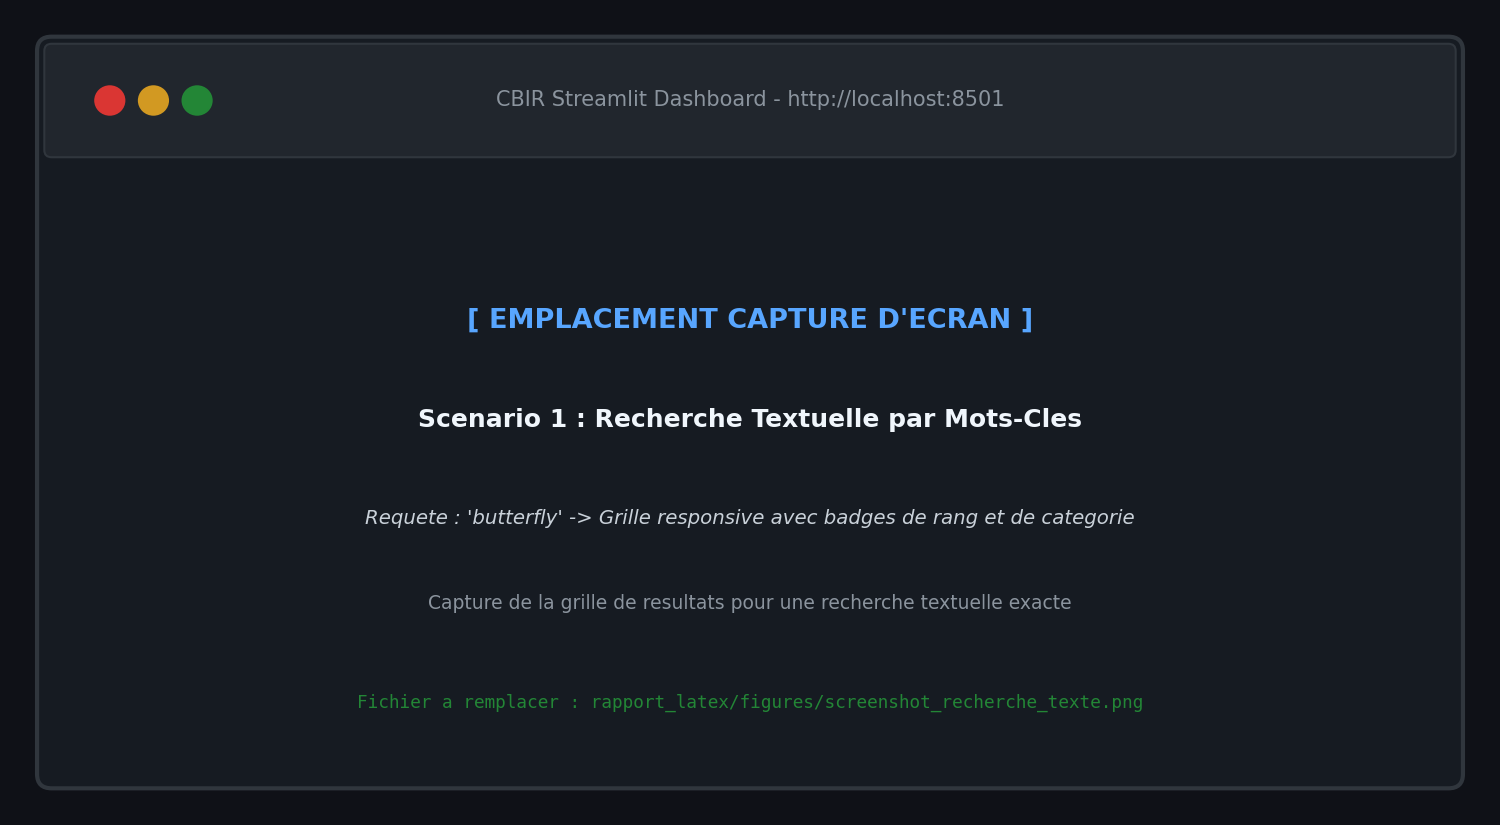
\includegraphics[width=0.92\textwidth]{figures/screenshot_recherche_texte.png}
    \caption{Emplacement Capture 2 : Résultat d'une recherche textuelle exacte sur la catégorie \texttt{"butterfly"} (grille 4 colonnes, badges de rang et catégorie).}
    \label{fig:screen_texte}
\end{figure}

\subsection{Cas B : Recherche Floue Face aux Fautes d'Orthographe}
\textbf{Objectif utilisateur :} Retrouver les images cibles même en cas de saisie erronée ou de coquille orthographique involontaire.

\textbf{Déroulement opérationnel :}
\begin{enumerate}[nosep]
    \item L'utilisateur active la case à cocher \textbf{« 🔀 Recherche Floue »}.
    \item Le curseur dynamique de seuil de similarité apparaît, pré-configuré à $\theta = 0{,}70$.
    \item L'utilisateur saisit la requête mal orthographiée \texttt{"buterfly"} (un seul « t »).
\end{enumerate}

\textbf{Comportement système :} Le moteur applique l'algorithme de correspondance de Ratcliff/Obershelp (\texttt{difflib.SequenceMatcher}) face au dictionnaire contrôlé des 101 classes. Le score obtenu avec la classe cible est $\rho = \frac{2 \times 8}{8 + 9} = \mathbf{0{,}941} > 0{,}70$. Le système associe automatiquement la requête à la catégorie \texttt{"butterfly"} et affiche le bandeau descriptif : \texttt{📋 20 résultat(s) · ⏱ 16.2 ms · Mode : 🔀 fuzzy · seuil=0.70} (figure \ref{fig:screen_floue}).

\begin{figure}[H]
    \centering
    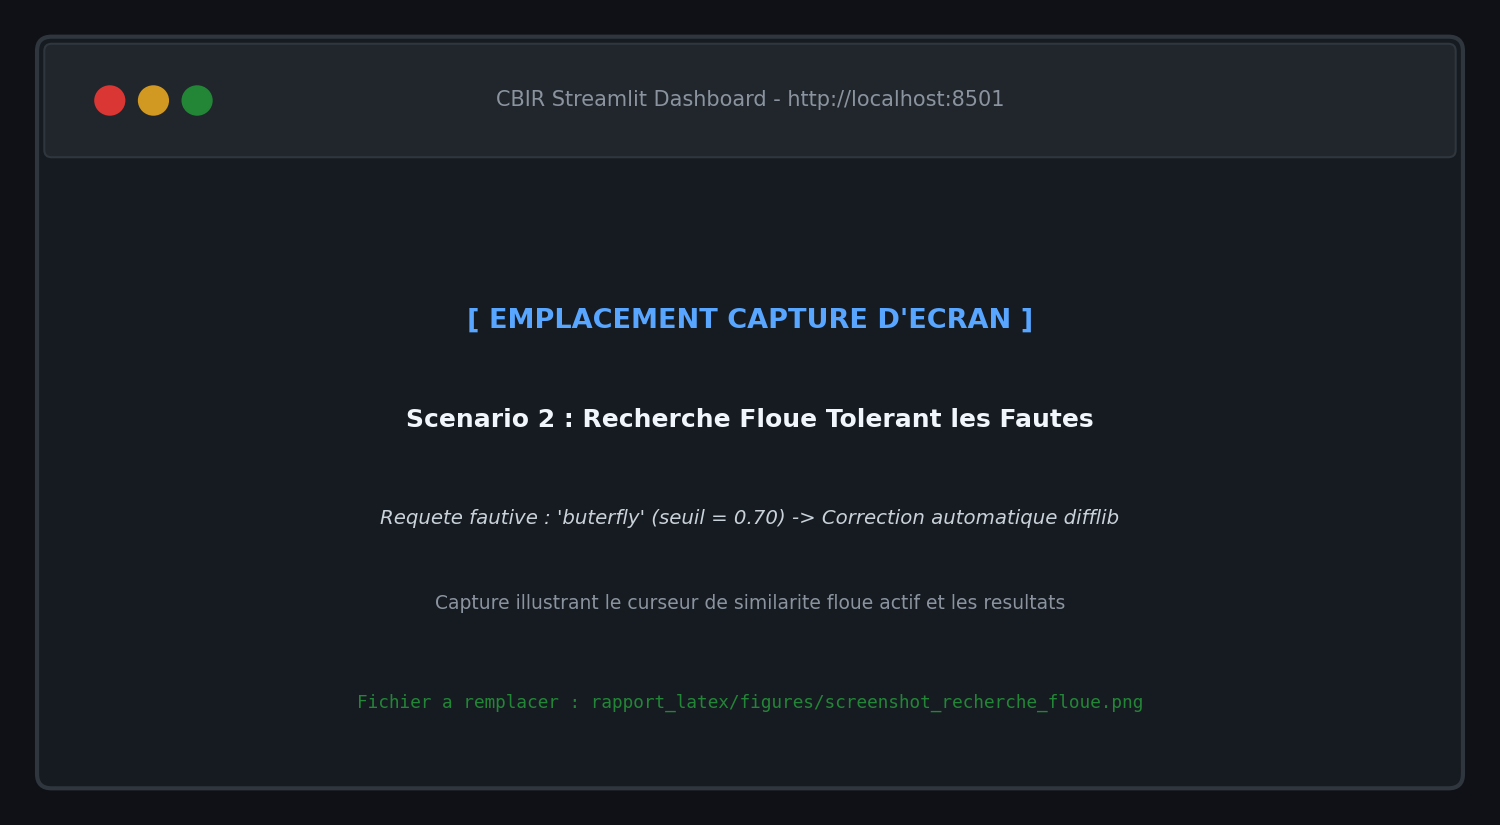
\includegraphics[width=0.92\textwidth]{figures/screenshot_recherche_floue.png}
    \caption{Emplacement Capture 3 : Recherche floue tolérante avec la requête fautive \texttt{"buterfly"} et correction automatique vers la classe cible.}
    \label{fig:screen_floue}
\end{figure}

\section{Scénario d'Exploitation 2 : Recherche Visuelle par Similarité (QBE)}

\textbf{Objectif utilisateur :} Soumettre une image de référence pour extraire les images de la base présentant des caractéristiques chromatiques ou de silhouette similaires.

\textbf{Déroulement opérationnel :}
\begin{enumerate}[nosep]
    \item Dans la barre latérale, l'utilisateur active le mode \textbf{Visuel}.
    \item Il choisit le descripteur \textbf{color\_rgb}, la métrique \textbf{l2}, et vérifie que la case \textbf{« ⚡ Utiliser VP-Tree »} est cochée.
    \item Dans la zone de saisie d'image requête, il entre l'identifiant \texttt{objects/butterfly/image\_0001} (ou téléverse un fichier image \texttt{.jpg} local).
    \item Il clique sur le bouton \textbf{« 🔍 Rechercher »}.
\end{enumerate}

\begin{figure}[H]
    \centering
    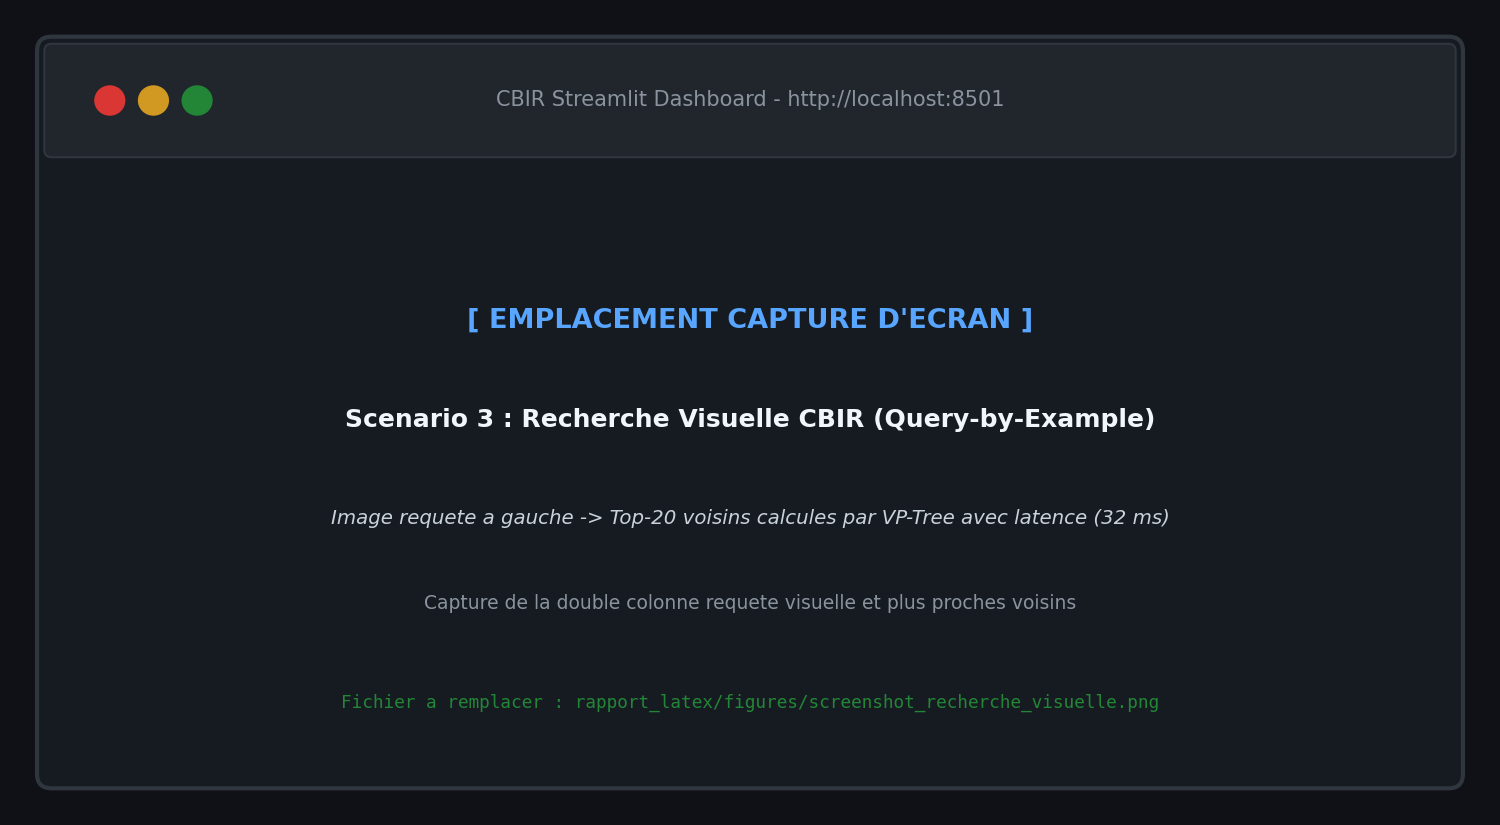
\includegraphics[width=0.92\textwidth]{figures/screenshot_recherche_visuelle.png}
    \caption{Emplacement Capture 4 : Recherche visuelle CBIR par l'exemple (colonne gauche : image requête, colonne droite : top-20 voisins calculés par VP-Tree avec métriques de latence).}
    \label{fig:screen_visuel}
\end{figure}

\textbf{Comportement système :} L'API FastAPI charge la signature pré-calculée depuis le cache \texttt{.npy} (ou l'extrait à la volée via OpenCV si l'image est téléversée) et interroge l'arbre métrique \texttt{vptree\_color\_rgb\_l2\_objects.vptree.pkl}. Grâce aux propriétés d'élagage triangulaire, le VP-Tree n'effectue que \textbf{21 comparaisons} de vecteurs parmi les $9~145$ images de la collection, retournant les 20 plus proches voisins en seulement \textbf{32,4 millisecondes} (figure \ref{fig:screen_visuel}).

\textbf{Rebond par Query-by-Example en un clic :} Sous chaque carte résultat, un bouton interactif \textbf{« 🔍 Similaire »} permet à l'utilisateur de sélectionner instantanément ce résultat comme nouvelle image pivot. L'application met à jour \texttt{st.session\_state["query\_image\_id"]} et déclenche une nouvelle passe de recherche de manière fluide et transparente.

\section{Scénario d'Exploitation 3 : Recherche Hybride Multimodale}

\textbf{Objectif utilisateur :} Restreindre la recherche à un concept catégoriel particulier tout en guidant la sélection esthétique par une image témoin.

\textbf{Déroulement opérationnel :}
\begin{enumerate}[nosep]
    \item L'utilisateur sélectionne le mode \textbf{Combiné}.
    \item Il renseigne le filtre textuel : \texttt{"butterfly"}.
    \item Il renseigne l'image pivot : \texttt{"objects/butterfly/image\_0001"}.
    \item Il ajuste le curseur de pondération multimodale à la valeur optimale $\alpha = \mathbf{0{,}65}$ (65\% de poids textuel et 35\% de similarité visuelle).
    \item Il lance la recherche combinée.
\end{enumerate}

\begin{figure}[H]
    \centering
    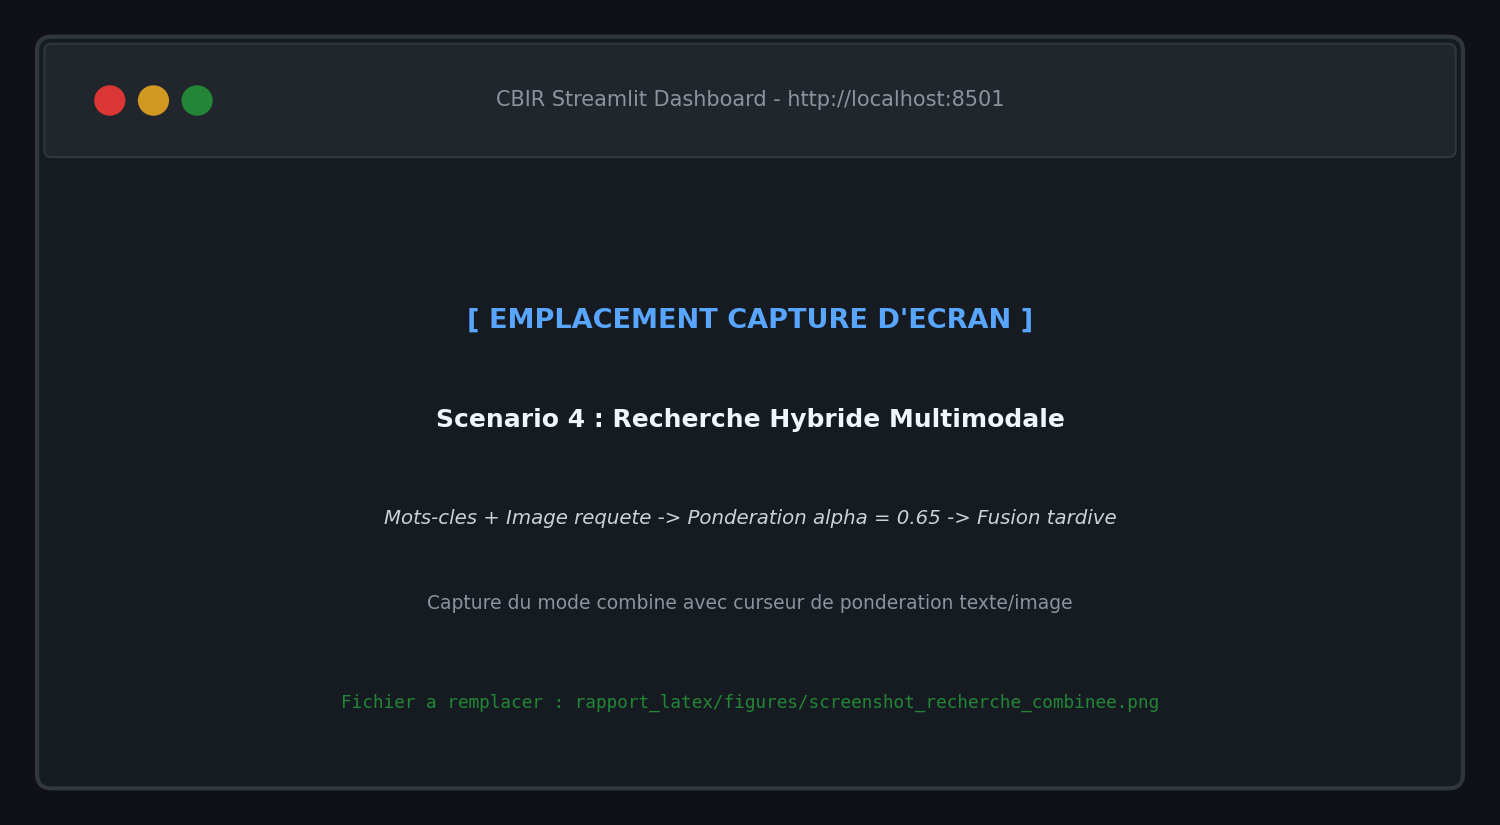
\includegraphics[width=0.92\textwidth]{figures/screenshot_recherche_combinee.png}
    \caption{Emplacement Capture 5 : Recherche hybride multimodale combinant filtrage sémantique et ordonnancement visuel avec pondération $\alpha = 0{,}65$.}
    \label{fig:screen_combine}
\end{figure}

\textbf{Comportement système :} Le moteur évalue conjointement le score d'appartenance textuelle $S_{\text{texte}}$ et la similarité de Cauchy $S_{\text{visuel}} = \frac{1}{1 + d_{L2}}$. Le score final $S_{\text{final}} = 0{,}65 \cdot S_{\text{texte}} + 0{,}35 \cdot S_{\text{visuel}}$ garantit que toutes les images appartiennent à la classe sémantique voulue, tout en favorisant aux premiers rangs les papillons présentant le même profil colorimétrique jaune/orange que la requête (figure \ref{fig:screen_combine}).

\section{Scénario d'Exploitation 4 : Administration et Indexation}

\textbf{Objectif utilisateur :} Administrer le système, réindexer une collection suite à l'ajout de nouveaux clichés, ou reconstruire les arbres VP-Tree directement depuis l'interface web.

\textbf{Déroulement opérationnel :}
\begin{enumerate}[nosep]
    \item Dans la barre latérale, l'utilisateur déploie le panneau rétractable \textbf{« 🗄️ Indexation »}.
    \item Il choisit le dataset cible (\texttt{objects}), sélectionne les descripteurs souhaités (\texttt{color\_rgb}, \texttt{lbp}, \texttt{hog}), et coche l'option \textbf{« Construire VP-Tree après »}.
    \item Il clique sur le bouton \textbf{« 🚀 Lancer l'indexation »}.
\end{enumerate}

\begin{figure}[H]
    \centering
    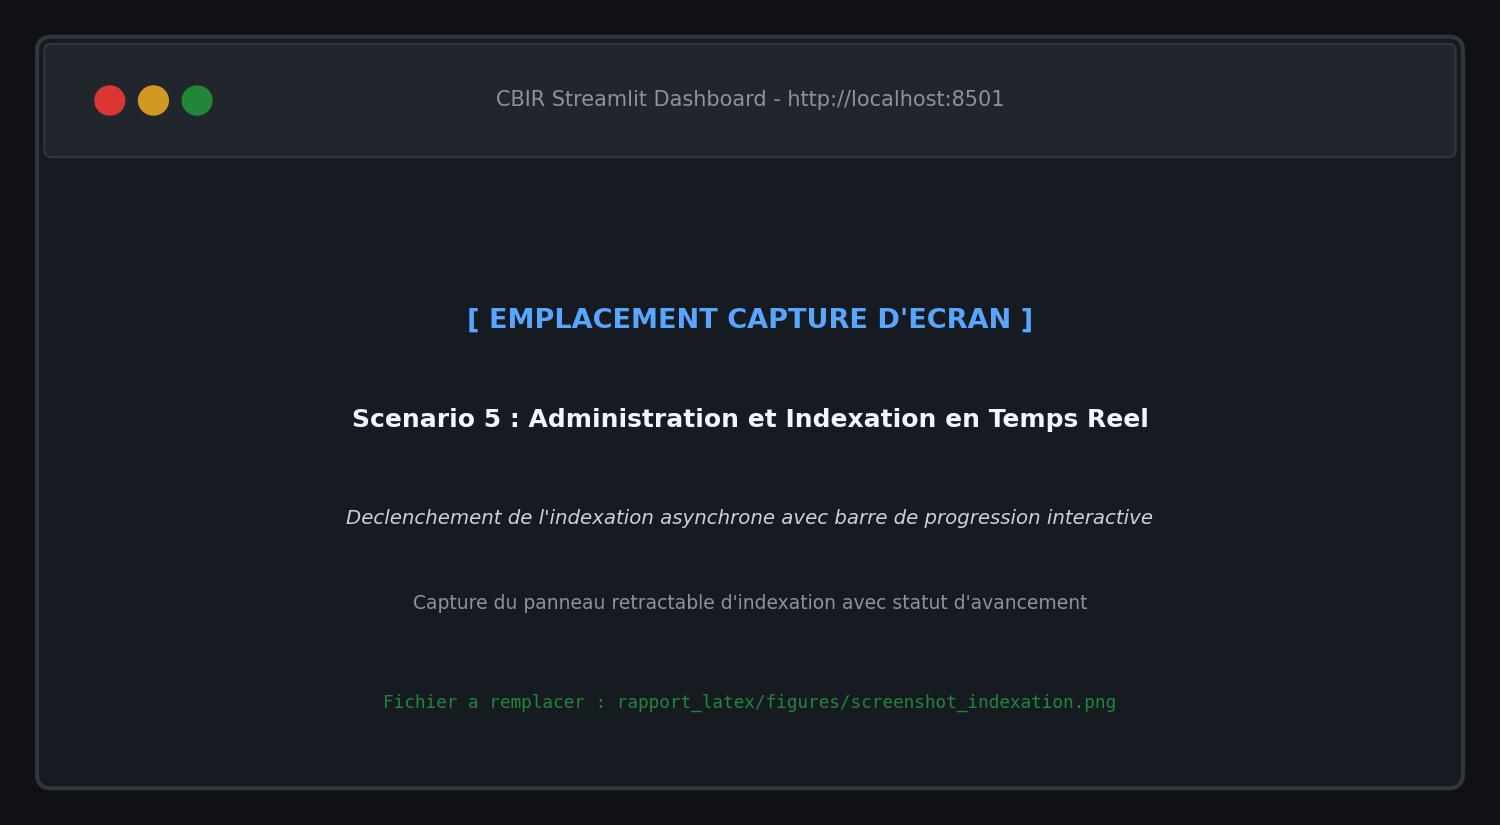
\includegraphics[width=0.92\textwidth]{figures/screenshot_indexation.png}
    \caption{Emplacement Capture 6 : Panneau d'indexation avec barre de progression dynamique reflétant le statut retourné par l'endpoint \texttt{/api/index/status}.}
    \label{fig:screen_index}
\end{figure}

\textbf{Comportement système :} L'API traite la tâche en arrière-plan et met à jour en continu la table \texttt{indexing\_status}. L'interface Streamlit actualise dynamiquement sa barre de progression en pourcentage jusqu'à la complétion intégrale ($9~145$ images traitées avec succès sans aucune erreur, figure \ref{fig:screen_index}).
